\documentclass[a4paper,11.5pt,]{article}
\usepackage[utf8]{inputenc}
\usepackage[T1]{fontenc,url}
\usepackage[english,]{babel}
\usepackage{blindtext}
\usepackage{natbib}
\usepackage{gensymb}
\usepackage{amsmath}
\usepackage{changepage}
\usepackage{mathabx}
\usepackage{amssymb}
\usepackage{commath}
\usepackage{physics}
\usepackage{multicol}
\usepackage{float}
\usepackage{listings}
\usepackage{graphicx}
\usepackage{hyperref}
\usepackage{svg}
\usepackage{wrapfig}

\newenvironment{Figure}
  {\par\medskip\noindent\minipage{\linewidth}}
  {\endminipage\par\medskip}

\usepackage{multicol}
%\setlength{\columnsep}{1cm}

\usepackage{geometry}
 \geometry{
 a4paper,
 total={170mm,257mm},
 textheight =  592mm,
 left=15mm,
 right=15mm,
 tmargin=20mm,
 bmargin=20mm
 }
 \setlength{\columnsep}{20pt}
          

 \title{Stellar Spectra B. - LTE Line Formation\\
 AST4310}
 \date{\normalsize{23. November 2018} }
 \author{\textsc{\small{Metin San}}}
 
 
\begin{document}

\maketitle
\begin{center}
   \textsc{\url{https://github.com/MetinSa/AST4310/tree/master/SSB}}. 
\end{center}

\begin{center}
\textsc{Introduction}
\end{center}

\begin{adjustwidth}{1.5cm}{1.5cm}
In this report we will look at the formation of spectral lines in the solar atmosphere assuming Local Thermodynamical Equilibrium (LTE). We will build on the knowledge acquired through SSA where we studied spectral lines and their formation through the application of statistical methods. The report will consist of three parts. In the first part we will study the radial stratification of the solar atmosphere based on the standard model FALC. The second part will consider the continuous spectrum from the solar atmosphere with a focus on its formation. The final part will consider the formation of spectral lines in the solar spectrum with a focus on the Na I D$_1$ line. The programs used to create the following presented figures and results can be found on my Github through the link below the author name.
\end{adjustwidth}


\begin{multicols}{2}

\begin{center}
\textsc{1. Stratification of the solar atmosphere}
\end{center}

We begin our study by investigating the stratification of the solar atmosphere using the FALC model developed by Fontela et al. in 1993. The model is based on the assumption that the atmosphere is horizontally homogeneous and constant in with time (hydrostatic equilibrium).
We will now present some figures created using the FALC model along with data from the sun and discuss the observed features.

\begin{figure}[H]
    \centering
    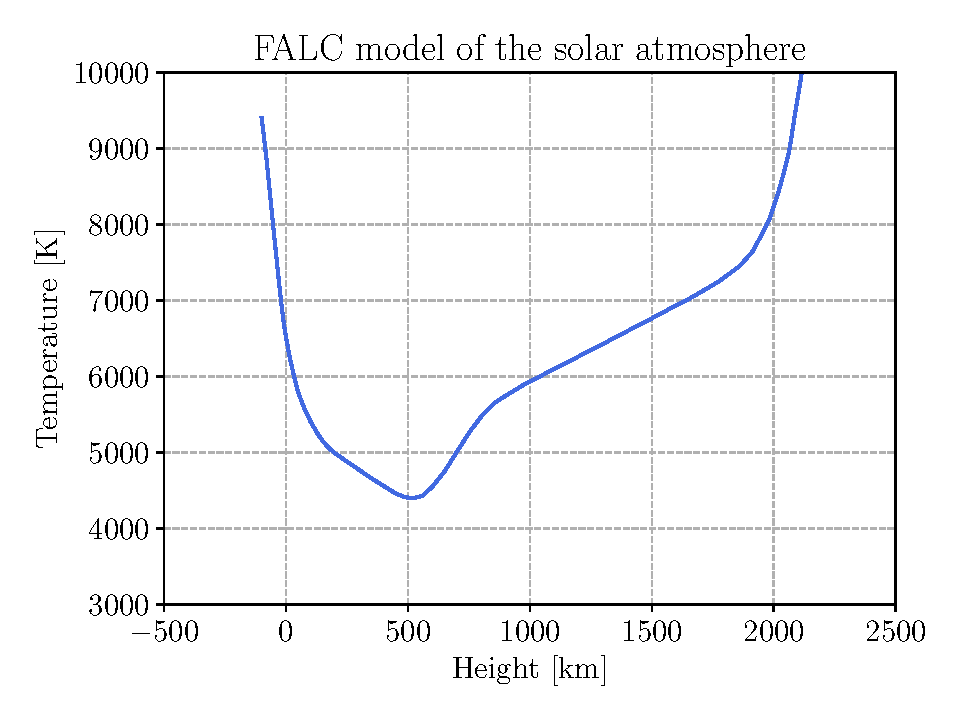
\includegraphics[width = 0.5\textwidth]{figures/1.2/FALCsolar_atmosphere.pdf}
    \caption{Recreation of the solar atmosphere stratification using the FALC model.}
    \label{fig: FALC atmo}
\end{figure}

 In figure \ref{fig: FALC atmo} we note that the temperature drops rapidly as we approach the "surface". The temperature experiences a minimum at height  $\approx 525$km which marks the end of the photosphere. We then move into the chromosphere where the temperature starts to increase. At heights around $\approx 2100$ we observe a steep increase. This is the transition region between the chromosphere and corona.

\begin{figure}[H]
    \centering
    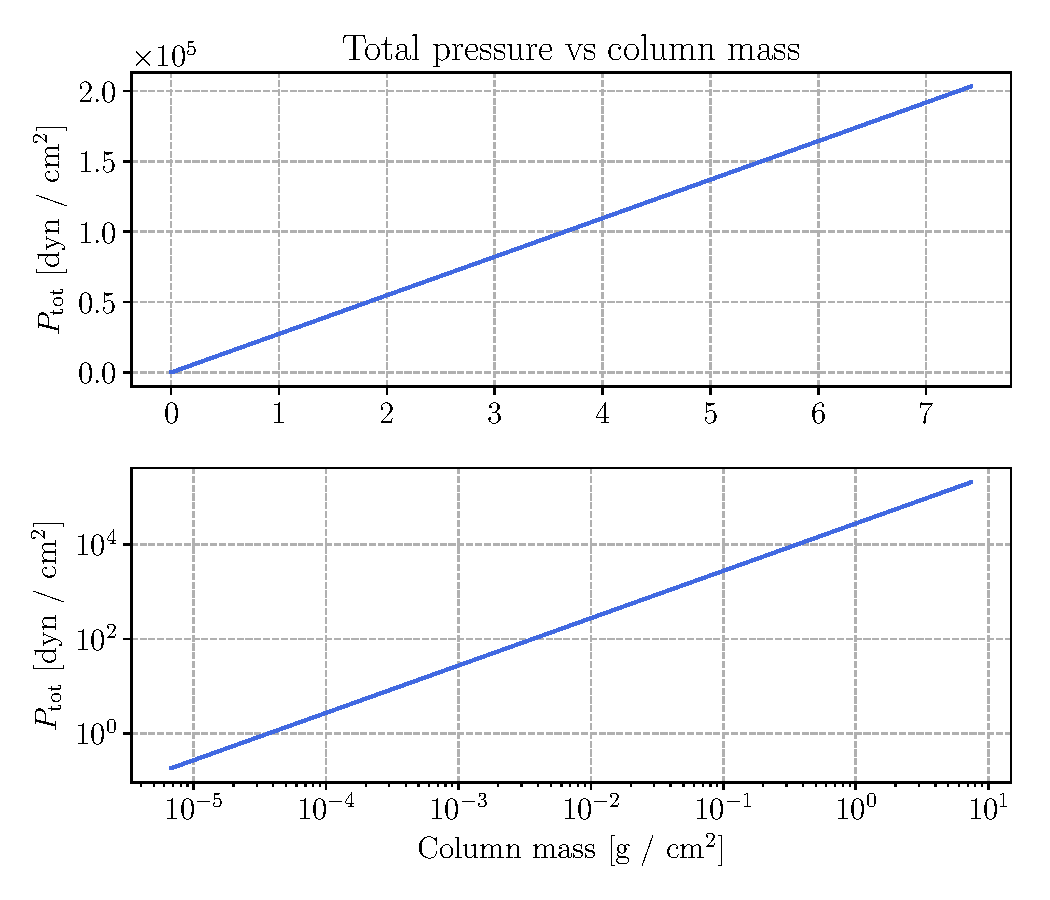
\includegraphics[width = 0.5\textwidth]{figures/1.2/FALCpressurelarge.pdf}
    \caption{The upper plot shows the total pressure $P_\mathrm{tot}$ plotted as a function of the column mass. The lower plot displays the same results in a log-log plot. The observed linearity allows us to express the total pressure as $P_\mathrm{tot} = Cm$, where $C$ is a constant and $m$ is the Column mass. By computing the average of $P/m$, we find that the constant $C = 2.74\times 10^4$ cm/s$^2$ = $g_\mathrm{surface}$ is the solar surface gravity. This is a result of the atmosphere being in hydrostatic equilibrium.}
    \label{fig: FALC P_tot/m}
\end{figure}

\begin{figure}[H]
    \centering
    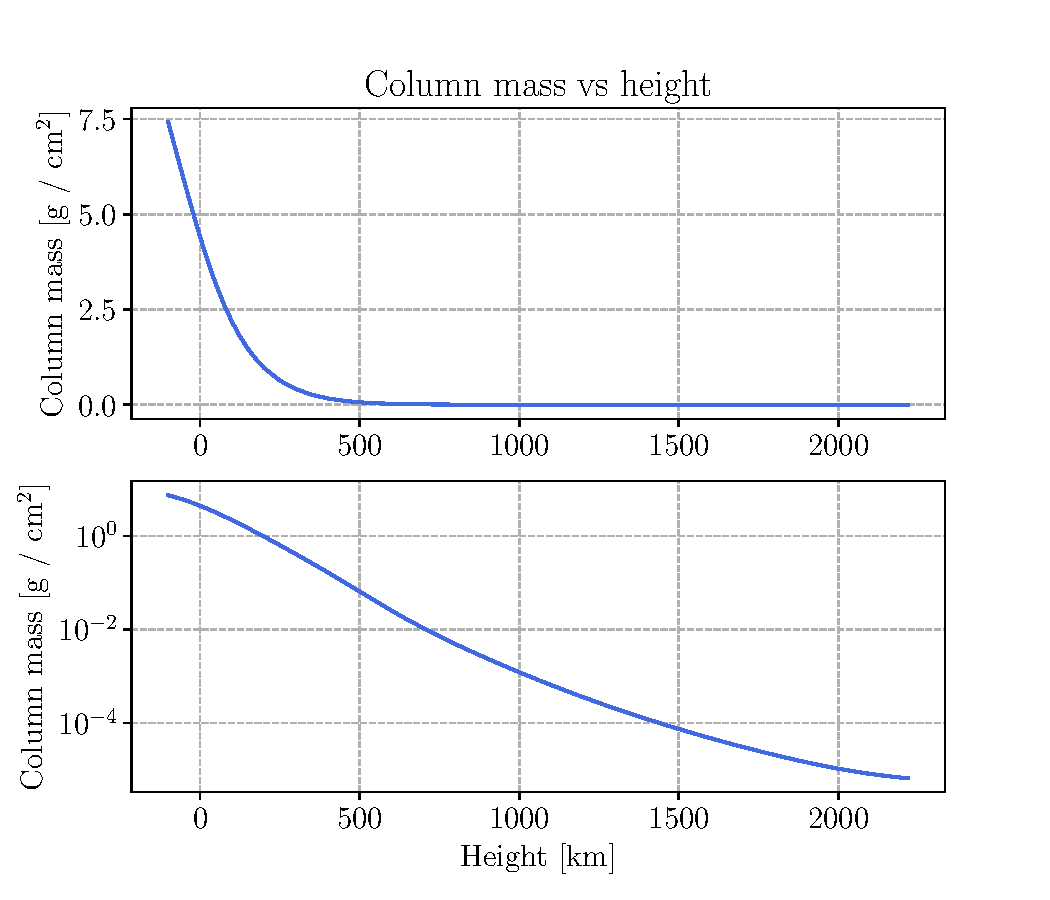
\includegraphics[width = 0.5\textwidth]{figures/1.2/FALCcolumnmass_heightlarge.pdf}
    \caption{The upper plot shows the column mass plotted against height. The lower plot shows the same results in a log-y plot. The near linearity suggests that the change in column mass with respect to height is nearly constant. We do observe a slight non-linearity in the low photosphere and also in the transition region between the chromosphere and corona. This is likely due to the different circumstances present at these locations, such as very high temperatures.}
    \label{fig: FALC m/h}
\end{figure}

\begin{figure}[H]
    \centering
    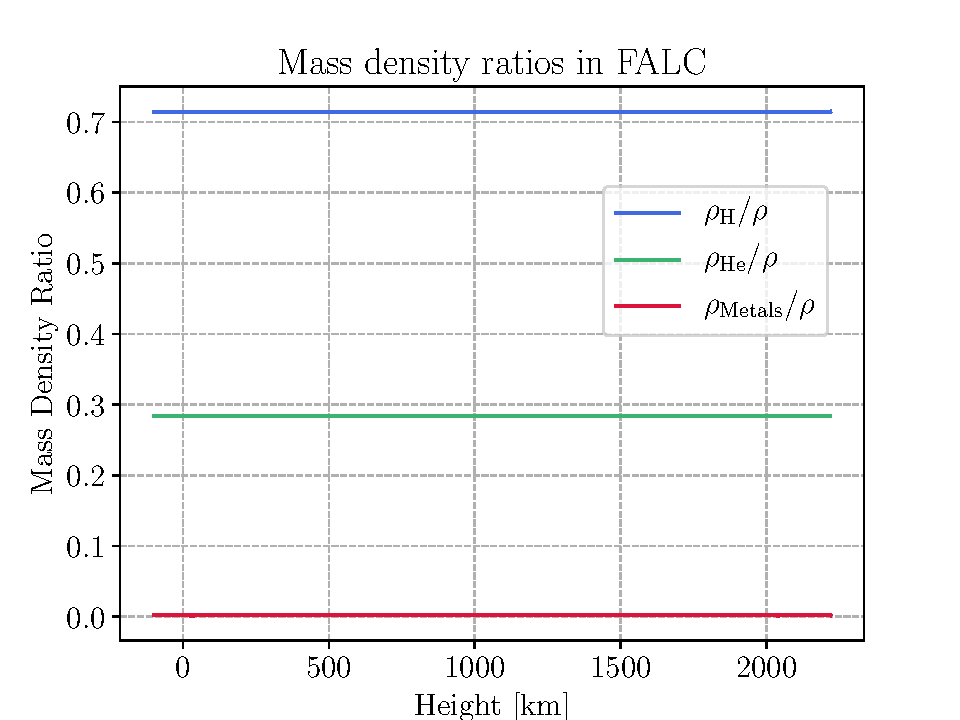
\includegraphics[width = 0.5\textwidth]{figures/1.2/FALCmassdensity.pdf}
    \caption{Mass density ratios of hydrogen, helium and the metals. The different ratios sum to unity. We observe that the mass density ratios are independent of height. This is a result of the complete mixing assumption made. }
    \label{fig: FALC abundance}
\end{figure}

\begin{figure}[H]
    \centering
    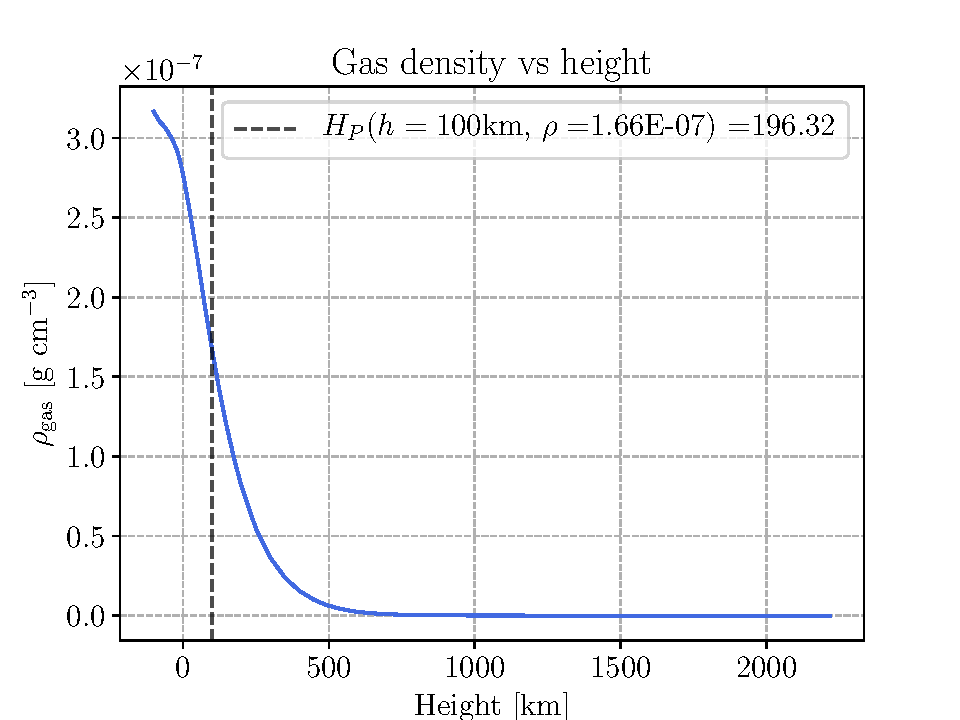
\includegraphics[width = 0.5\textwidth]{figures/1.2/FALCgasDensity.pdf}
    \caption{Gas density as a function of height. We observe that the gas density quickly approaches 0 as we move further away from the "surface". The density scale height $H_\rho$ can be derived from $\rho = \rho(0) \exp(-h/H_\rho)$. Inserting the height and density parameters at the deep photosphere border (denoted by the stippled line), we find that the density scale height is $H_\rho = 196.32$km.}
    \label{fig: FALC gasdens}
\end{figure}

\begin{figure}[H]
    \centering
    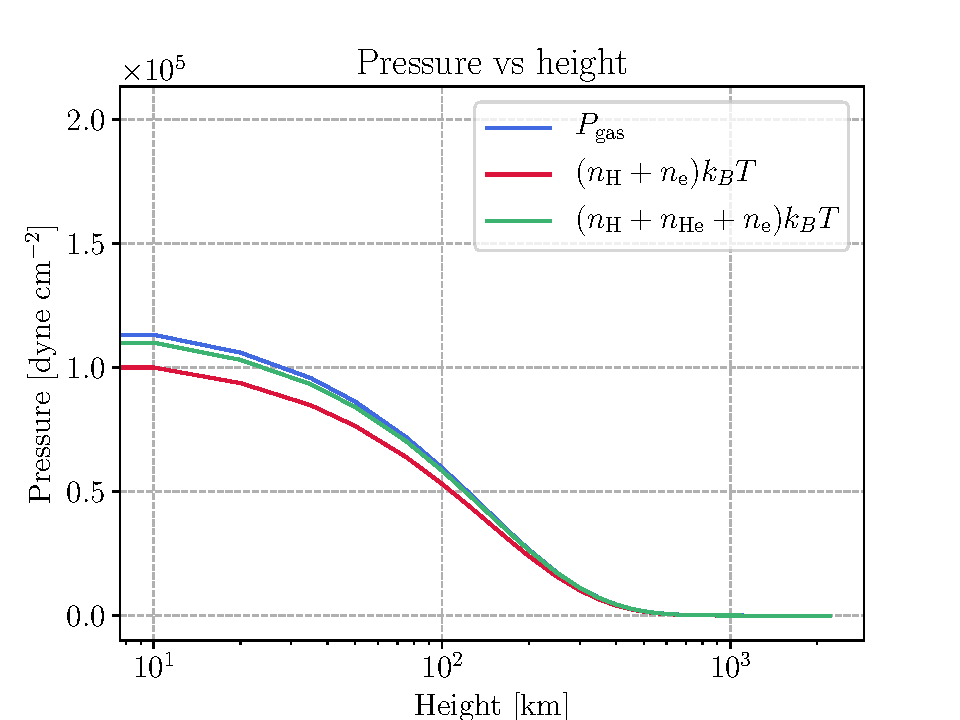
\includegraphics[width = 0.5\textwidth]{figures/1.2/FALCgasPressure.pdf}
    \caption{Pressure plotted against height. The gas pressure is plotted along side two ideal gas approximations, $(n_\mathrm{H} + n_\mathrm{e})k_B T$, and $(n_\mathrm{H} + n_\mathrm{He} + n_\mathrm{e})k_B T$. We note that the ideal gas approximation with the addition of the helium number density is the better approximation. This is because the amount of helium in the sun is non negligible and should definitely be considered. }
    \label{fig: FALC p/h}
\end{figure}

\begin{figure}[H]
    \centering
    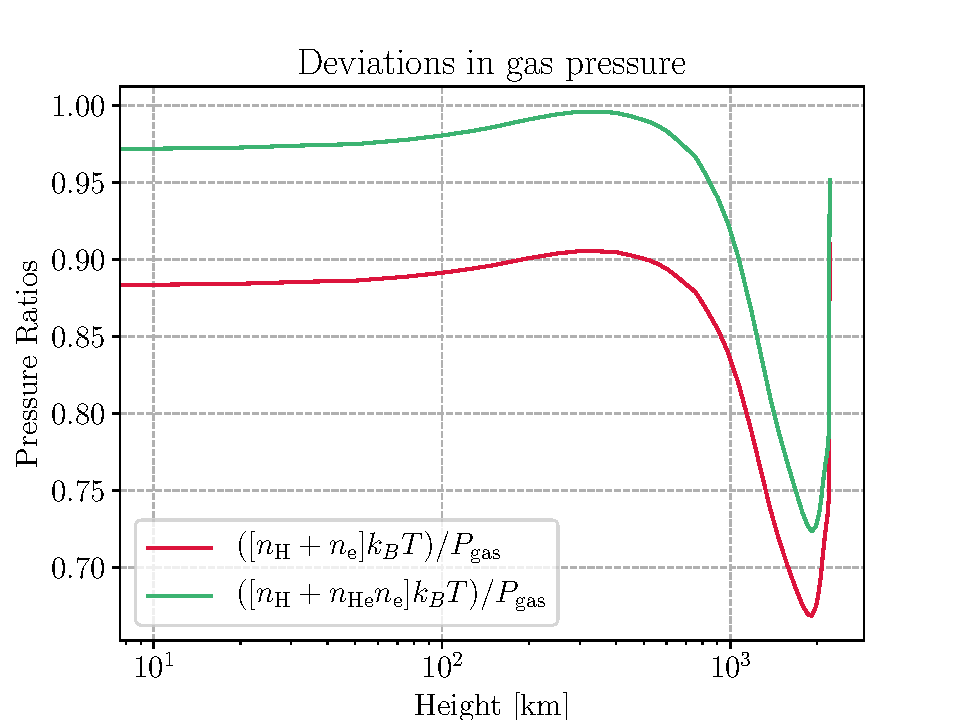
\includegraphics[width = 0.5\textwidth]{figures/1.2/FALCgasPressureDeviations.pdf}
    \caption{The ratios between the gas pressure and the ideal gas approximations seen in figure \ref{fig: FALC p/h} as functions of height. We observe that the deviation is much larger for the approximation without helium. At heights around $\approx 1300$km, we observe a near perfect ideal gas approximation. The deviation of both approximations increase as we approach the transition region to the corona. }
    \label{fig: FALC dev}
\end{figure}


\begin{figure}[H]
    \centering
    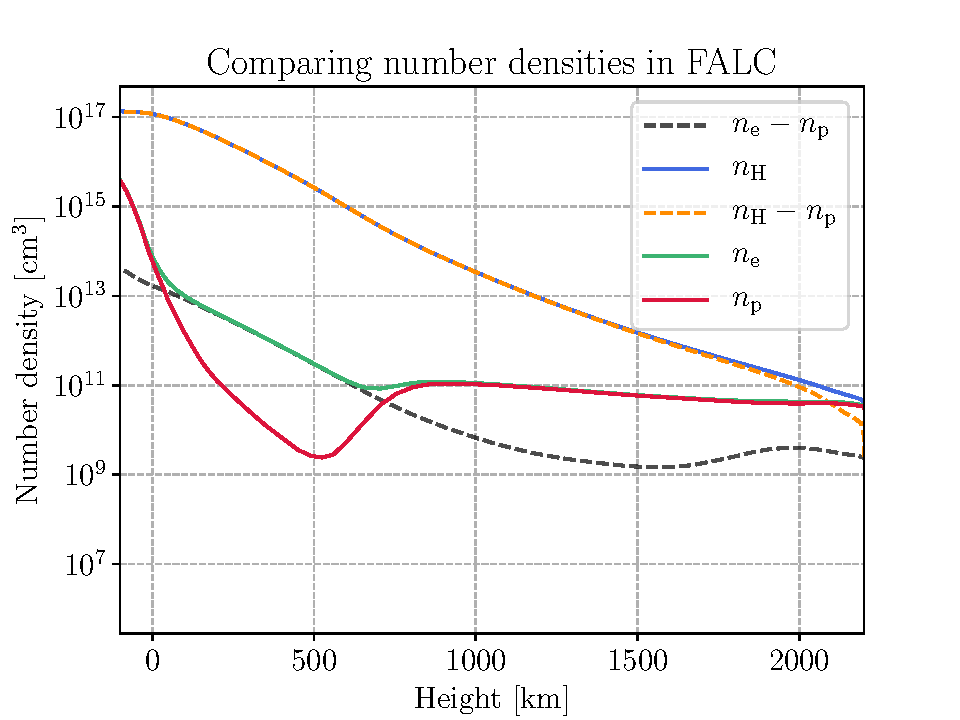
\includegraphics[width = 0.5\textwidth]{figures/1.2/FALCnumberDensity.pdf}
    \caption{The total hydrogen, proton and electron number densities as a function of height. We have also plotted $n_H - n_p$ which is the number of electrons that do not result from hydrogen ionization. We note that $n_H - n_p$ are parallel to $n_e$ through most of the height range. As we approach the transition region to the corona, temperatures increase so much that hydrogen starts to get ionized which results in the deviation of the two curves. We have also plotted the electrons coming from metals in $n_e - n_p$.
    We note that all electrons originate from metals (species other than hydrogen) at heights ranging from $0 - 600$km. This explains the metal spectral lines observed in the solar spectra as this is the height in which most of the spectral lines form. }
    \label{fig: FALC number densities}
\end{figure}

A final study for the FALC model is to compare the particle density with the photon density. We can find the photon density in the FALC model from the equation
\begin{figure}[H]
    \centering
    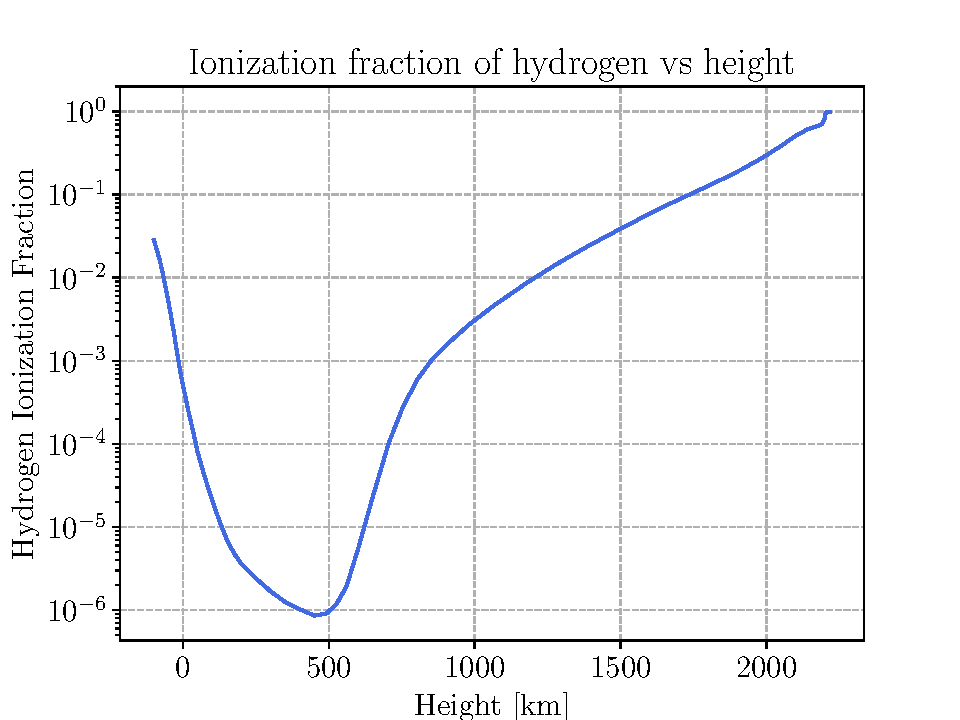
\includegraphics[width = 0.5\textwidth]{figures/1.2/FALCIonizationFraction.pdf}
    \caption{The ionization fraction of hydrogen as a function of height plotted in log-y. We notice that this very much resembles the temperature of the seen in figure \ref{fig: FALC atmo}. This is because the ionization is heavily temperature dependant, so the curve follows the behaviour of the temperature. Note that at the transition region to the corona, the ionization fraction approaches 1. This explains some of the behaviour discussed in the number densities in figure \ref{fig: FALC number densities}.}
    \label{fig: FALC ionization}
\end{figure}


\begin{equation}\label{eq:1}
    N_\mathrm{photon} \sim 20T^3,
\end{equation}
where we have again assumed thermodynamical equilibrium. High up in the atmosphere , the photon density can be approximated as 

\begin{equation}\label{eq:2}
    N_\mathrm{photon}^{\mathrm{top}} = \frac{20}{2\pi}T_{eff}^3,
\end{equation}
where $T_\mathrm{eff} = 5440$K. By using equation \eqref{eq:2}, we find that the photon density at the highest model location(height $\approx 2200$km) is $N_\mathrm{photon}^{\mathrm{top}} = 6 \times 10^{12}$cm$^{-3}$. We can compare this with the previously computed particle number densities, where we find that the number density of hydrogen at the highest model location is $n_\mathrm{H} = 5.57 \times 10^9$cm$^{-3}$. 

Similarly, for the deepest model location(height$ = -100$km) we find the following values for the densities $N_\mathrm{photon} = 1.66 \times 10^{13}$cm$^{-3}$, and $n_\mathrm{H} = 1.35 \times 10^{17}$cm$^{-3}$.

\begin{center}
    \textit{Comparison to Earth's atmosphere}
\end{center}

The FALC model can then be compared to measurements done on the Earth's atmosphere. Below is a set of figures describing some of the above studied quantities for Earth's atmosphere.

In figure \ref{fig: norm dens press} we notice that both the pressure and density behave mostly the same as a function of height. This is likely a result of their connection through the equation of state.

In figure \ref{fig: mu} we observe that the quantity is varying a lot for the first 100 km. This is probably as a result of the variations in the atmosphere. For higher heights it decreases as a result of the high atmosphere being dominated by lighter atoms. 

\begin{figure}[H]
    \centering
    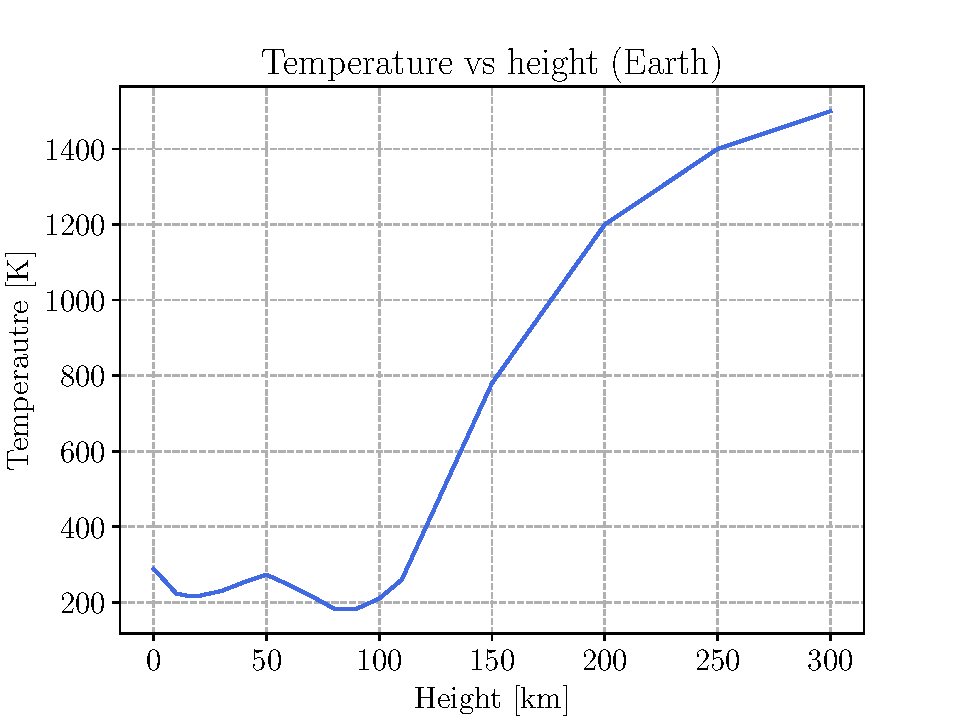
\includegraphics[width = 0.5\textwidth]{figures/1.3/Earth_temperature.pdf}
    \caption{Temperature of Earth's atmosphere as a function of height.}
    \label{fig: earth temp}
\end{figure}

\begin{figure}[H]
    \centering
    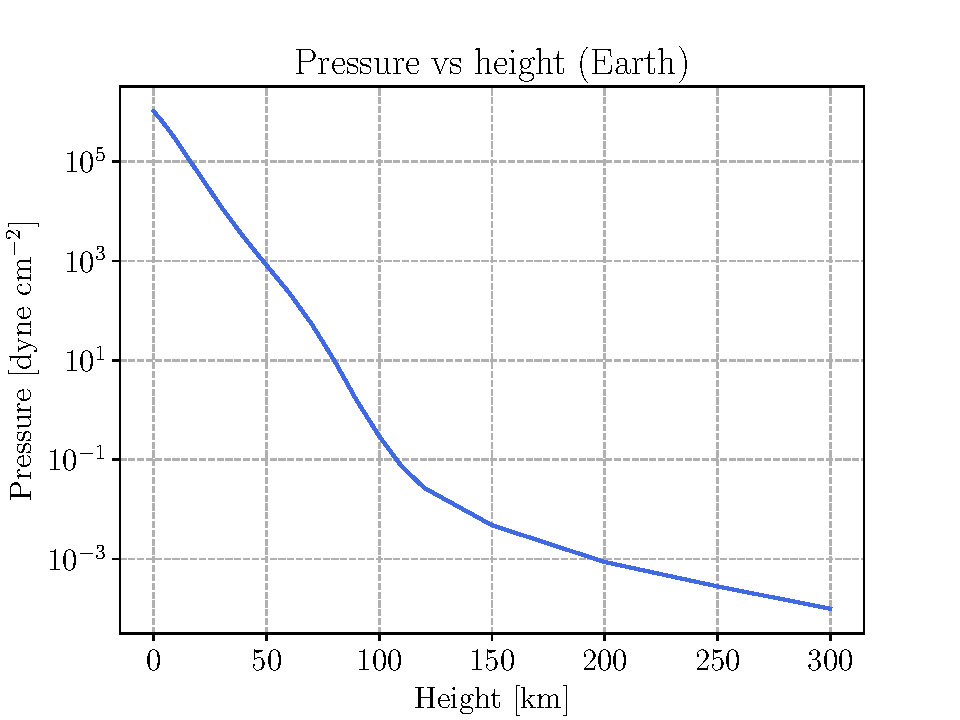
\includegraphics[width = 0.5\textwidth]{figures/1.3/Earth_pressure.pdf}
    \caption{The pressure of Earth's atmosphere as a function of height.}
    \label{fig: earth pressure}
\end{figure}

\begin{figure}[H]
    \centering
    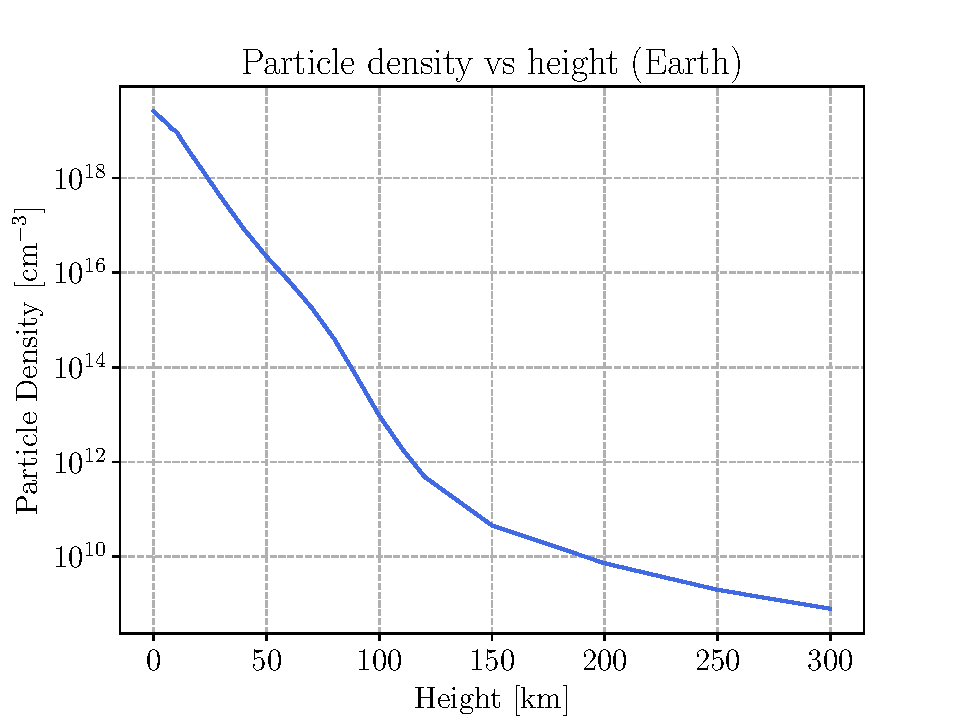
\includegraphics[width = 0.5\textwidth]{figures/1.3/Earth_particledensity.pdf}
    \caption{Particle density of Earth's atmosphere as a function of height.}
    \label{fig: earth part dens}
\end{figure}

\begin{figure}[H]
    \centering
    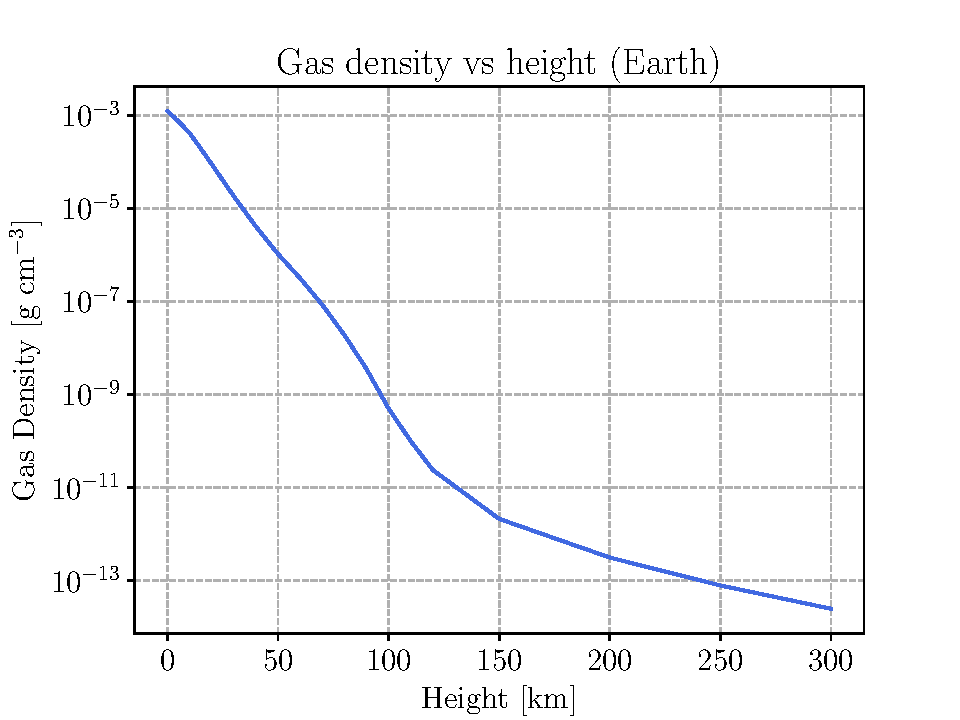
\includegraphics[width = 0.5\textwidth]{figures/1.3/Earth_gasdensity.pdf}
    \caption{The gas density of Earth's atmosphere as a function of height.}
    \label{fig: earth gas dens}
\end{figure}

\begin{figure}[H]
    \centering
    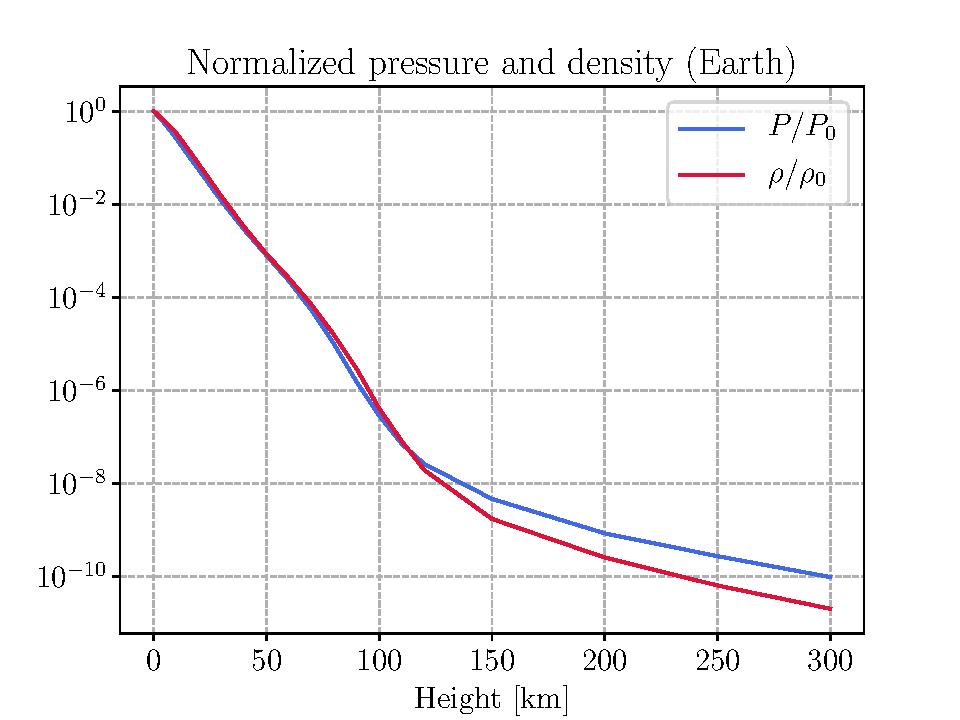
\includegraphics[width = 0.5\textwidth]{figures/1.3/Earth_Normalized_den_pres.pdf}
    \caption{The pressure and density of the Earth's atmosphere normalized with respect to their maximum value.} 
    \label{fig: norm dens press}
\end{figure}

\begin{figure}[H]
    \centering
    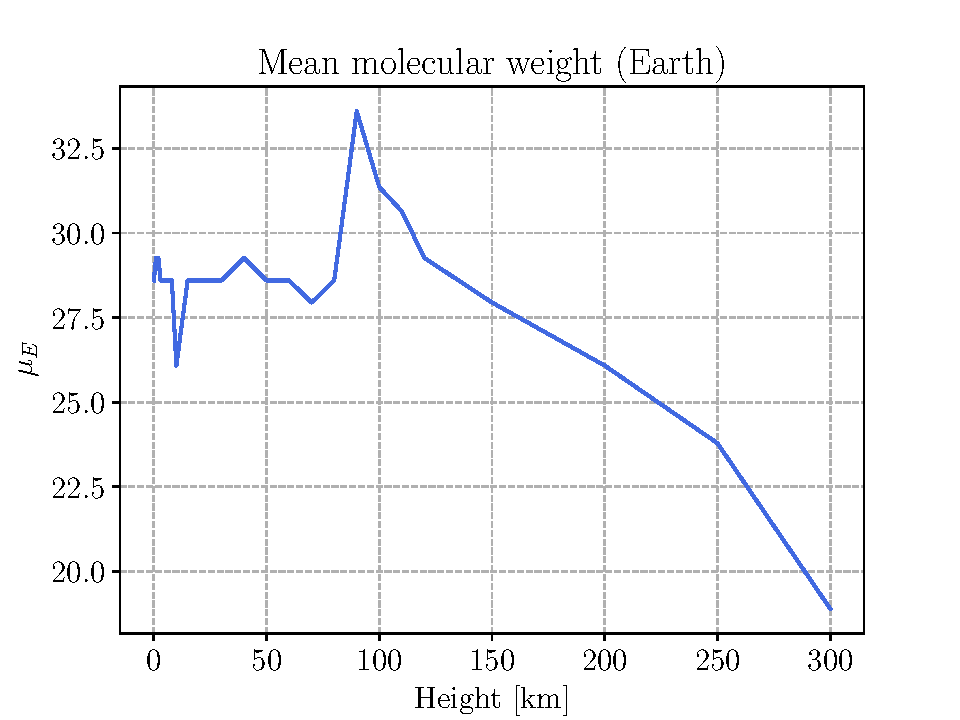
\includegraphics[width = 0.5\textwidth]{figures/1.3/Earth_mu.pdf}
    \caption{The mean molecular weight of Earth's atmosphere as a function of height.}
    \label{fig: mu}
\end{figure}

\begin{center}
2. \textsc{Continuous spectrum from the solar atmosphere}
\end{center}

This part considers the main section of the report. With the analysis of the FALC model done, we now move on to study the formation of the solar continuum, focusing on the visible and near-infrared parts. 

\begin{center}
2.1 \textit{Observed solar continua}
\end{center}

The data we have used in the coming analysis is provided by Allen (1976) and it specifies the continuum radiation emitted by the sun in the wavelengths of $\lambda \in [0.2,5]\mu$m with the spectral bandwidth $\Delta \lambda = 1 \mu$m. We will start by studying the two quantities: radially emergent intensity and astrophysical flux, in addition to their associated smoothed parts. 

The radially emergent continuum intensity $I_\lambda^\mathrm{cont}$ and the astrophysical continuum flux $F_\lambda^\mathrm{cont}$ share the same units of [erg cm$^{-2}$ s$^{-1}$ $\mu$m$^{-1}$ ster$^{-1}$], but they differ in that the flux is the net flow of energy, whereas the intensity is the flow of energy at a specific location in a specific direction. 

The four spectral distributions are plotted together in figure \ref{fig: Solar Cont}. We note that all distributions peak at around $0.5 \mu$ with slight deviations. The smoothed functions have decreased intensity peaks compared to their standard counterparts. These distributions can also be converted into the frequency bandwidth. Doing so and plotting the results as functions of wavelength gives us the frequency distribution seen in figure \ref{fig: Solar freq}.


\begin{figure}[H]
    \centering
    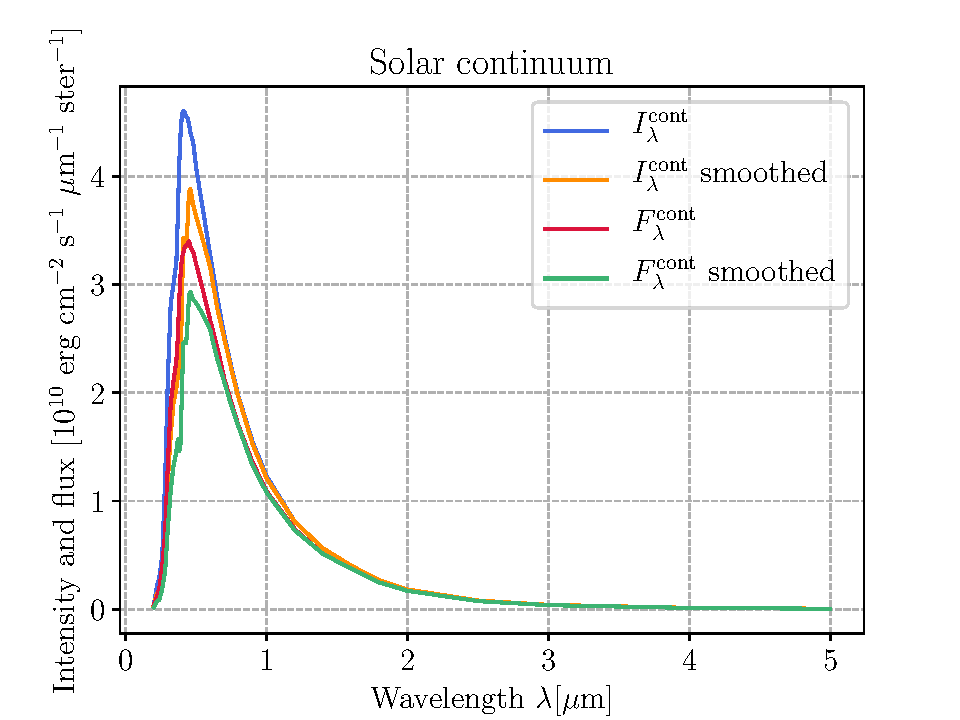
\includegraphics[width = 0.5\textwidth]{figures/2.1/solarcontinuum.pdf}
    \caption{Spectral distributions of the Sun as a function of wavelength in the range $\lambda \in [0.2,5]\mu$m.}
    \label{fig: Solar Cont}
\end{figure}

The emergent intensity from the sun can be approximated as black body radiation which is given by the Planck function

\begin{equation}\label{eq: Planck}
    B _ { \lambda } ( \lambda , T ) = \frac { 2 h c ^ { 2 } } { \lambda ^ { 5 } } \frac { 1 } { e ^{  h c / \lambda k _ {  B  } T } - 1},
\end{equation}

\begin{figure}[H]
    \centering
    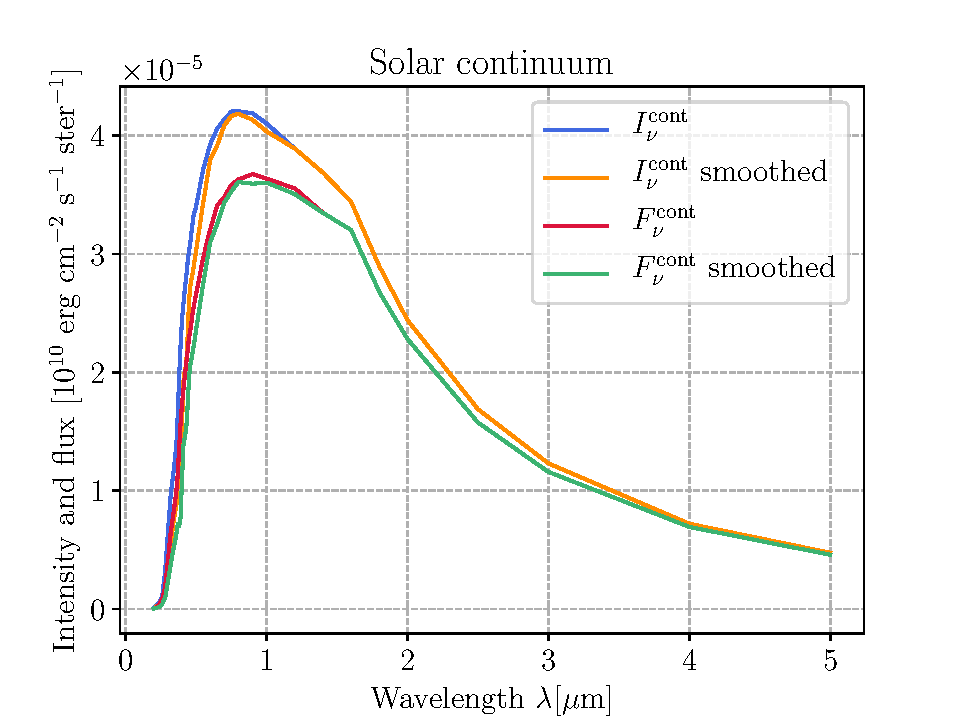
\includegraphics[width = 0.5\textwidth]{figures/2.1/solarcontinuum_freq.pdf}
    \caption{Spectral distributions of the Sun in the frequency bandwidth as a function of wavelength in the range $\lambda \in [0.2,5]\mu$m.}
    \label{fig: Solar freq}
\end{figure}

where $h$ is Planck's constant, $c$ is the speed of light, $k_B$ is the Boltzmann constant and $T$ is the temperature of the radiating black body.
We can then compute the Planck function for the same wavelength interval and compare the results to the observed intensity.

The results of this comparison is seen in figure \ref{fig: Planck} where we have made two Planck fits. The first fit has been made using the solar surface temperature $T = 5770$K. We note that this fit does not quite match the observed emergent intensity. A better approximation is seen with $T = 6300$k.

\begin{figure}[H]
    \centering
    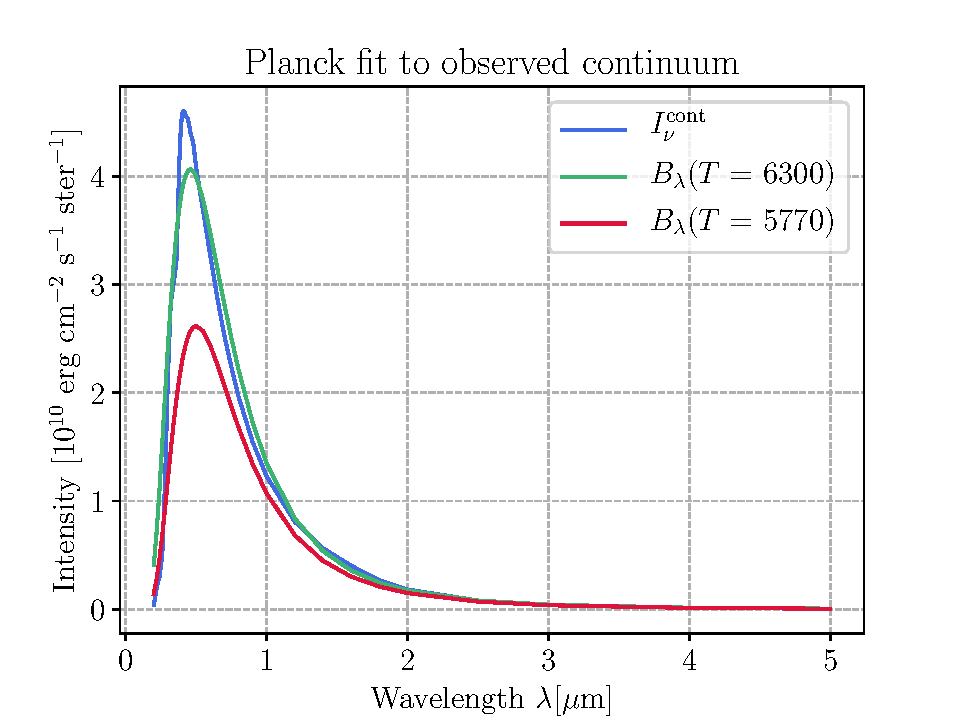
\includegraphics[width = 0.5\textwidth]{figures/2.1/solarcontinuum_planckfit.pdf}
    \caption{The fitting of two Planck curves of temperatures $T = 5770$K and $T = 6300$K to the emergent solar continuum intensity.}
    \label{fig: Planck}
\end{figure}

We can further invert the Planck function to obtain an expression for the brightness temperature $T_b$ which is defined as the temperature where $B_\lambda(T_b) \equiv I_\lambda$. Doing so gives us the expression

\begin{equation}\label{eq: bright}
    T _ { b } = \frac { h c } { k \lambda } \ln ^ { - 1 } \left( 1 + \frac { 2 h c ^ { 2 } } { I _ { \lambda } \lambda ^ { 5 } } \right).
\end{equation}
We can plot the brightness using the emergent intensity data. Doing so produces the results seen in figure \ref{fig: bright}. We observe that the brightness temperature peaks at $\lambda \approx 1.6 \mu$m which corresponds to radiation in the low infrared region of the spectrum. There is also another lower peak at $\lambda \approx 0.5\mu$m. This peak corresponds to green visual light. This is in accordance with the dominating color we know to receive from the sun. The peak at $\lambda = 1.6 \mu$m being the widest suggest that most of the energy transportation is through infrared radiation.


\begin{figure}[H]
    \centering
    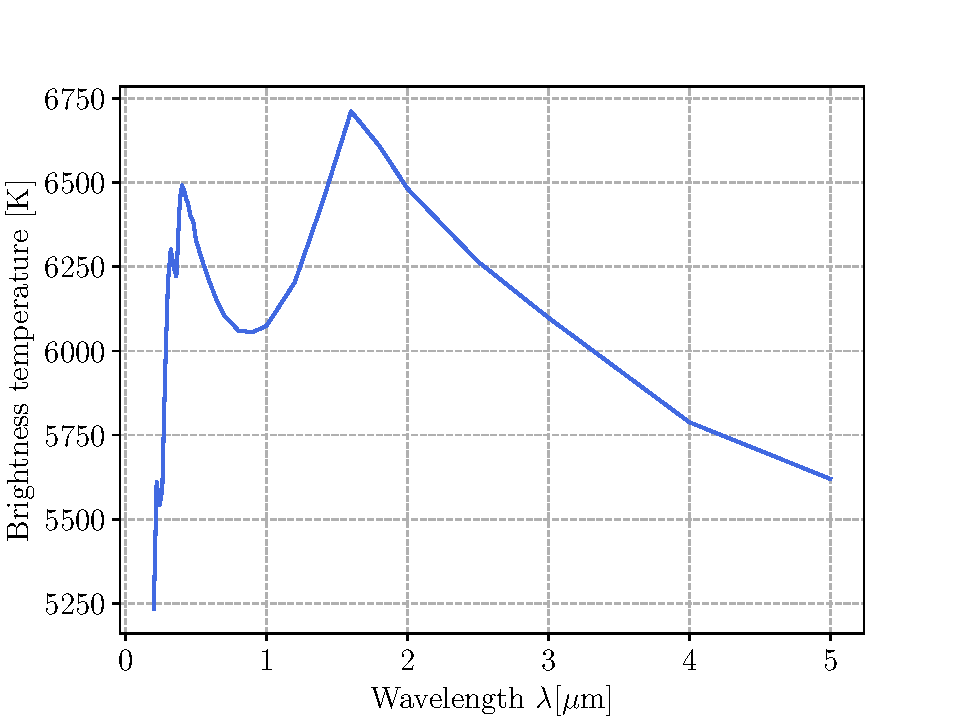
\includegraphics[width = 0.5\textwidth]{figures/2.1/solarcontinuum_brighttemp.pdf}
    \caption{The brightness temperature of the solar continuum. We observe two separate peaks in the temperature. The first being at $\approx 0.5 \mu$m. The second and higher peak is observed at $\approx 1.6 \mu$m.}
    \label{fig: bright}
\end{figure}

\begin{center}
2.2 \textit{Continuous extinction}
\end{center}

We will now move our attention over to extinction profiles. We will assume that H$^-$ is the major provider of continuous extinction in the solar atmosphere followed up by H I bound-free interactions. This is proves to be a good assumption for the solar photosphere for wavelengths $\lambda > 0.5 \mu$m. 

We implement the program \texttt{exthmin} provided by Gray (1992) in python. This program evaluates polynomial fits for H$^-$ extinction and delivers the total (bound-free + free-free) H$^-$ extinction in units of cm$^2$ per neutral hydrogen atom. This program allow us to plot the wavelength variation of the H$^-$ extinction for the FALC parameters at $h = 0$km. The results of this is seen in figure \ref{fig: H0}. The broad peak is caused by bound-free interactions, while the slope at $\lambda \gtrsim 1.6$ is a result of the free-free interactions.

The minimum observed at $\approx 1.6 \mu$m corresponds to the maximum brightness temperature. By inverting the results found in \ref{fig: H0}, we can therefore make the variation of H$^-$ extinction resemble the solar brightness temperature. This can be seen in figure \ref{fig: transmit}.


\begin{figure}[H]
    \centering
    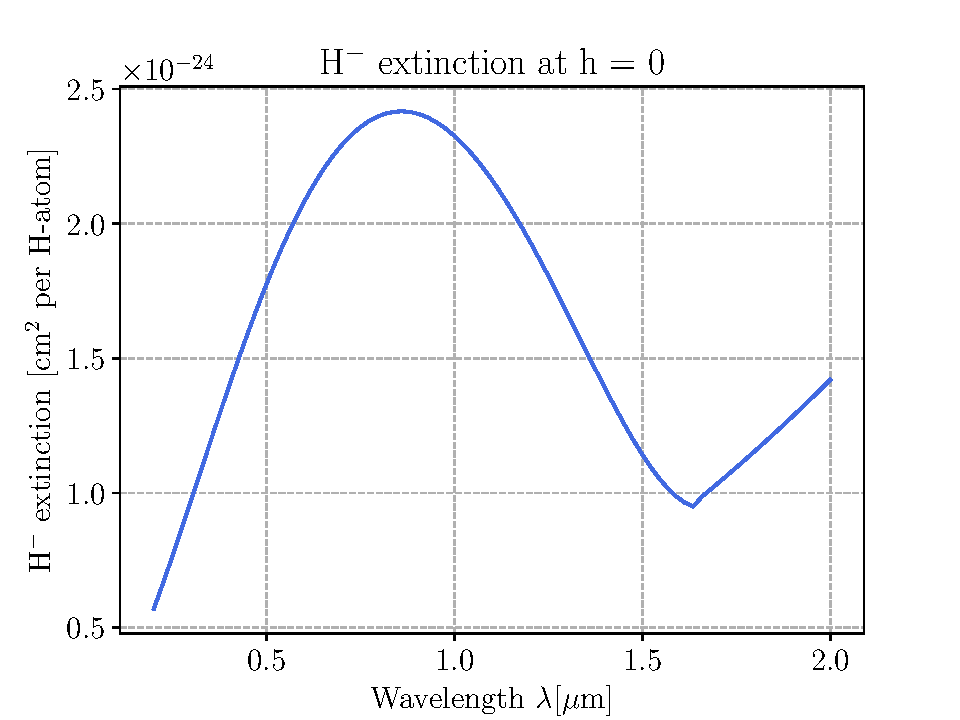
\includegraphics[width = 0.5\textwidth]{figures/2.2/extinction_H0.pdf}
    \caption{Varyation of H$^-$ extinction for the FALC parameters at $h=0$ in the solar atmoshpere as a function of wavelength.}
    \label{fig: H0}
\end{figure}

\begin{figure}[H]
    \centering
    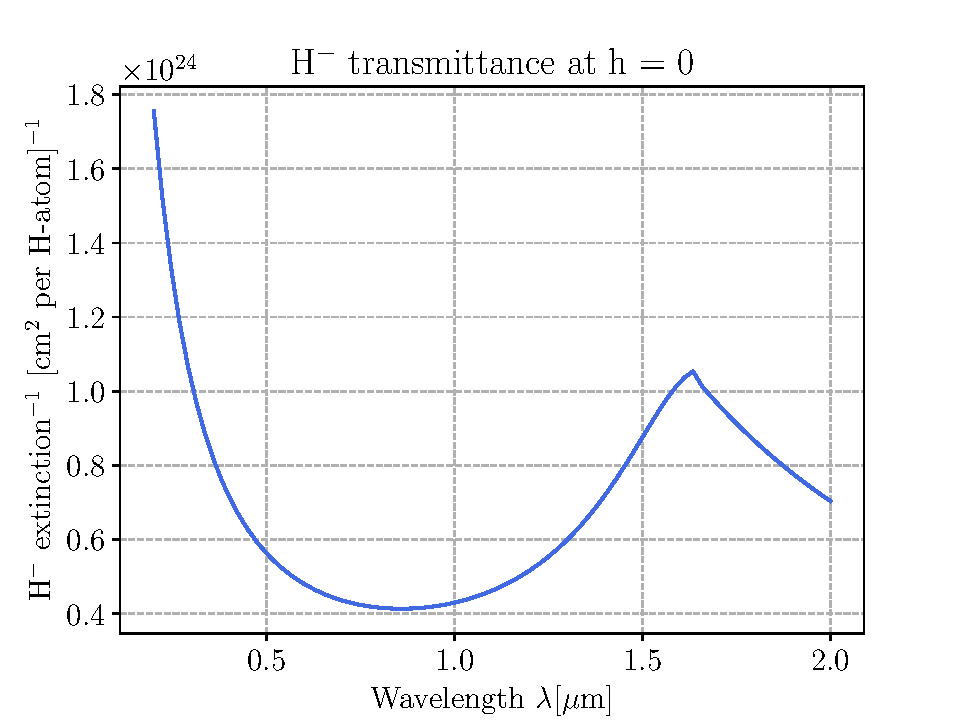
\includegraphics[width = 0.5\textwidth]{figures/2.2/extinction_transmittance.pdf}
    \caption{H$^-$ transmittance in the solar atmosphere at FALC parameters corresponding to $h=0$.}
    \label{fig: transmit}
\end{figure}

It is also interesting to study how the different extinction profiles behave at the different heights. This is done by using the data of the solar number densities provided by the FALC model. By multiplying the height-dependent results with $n_\mathrm{neutral\; H} \approx n_\mathrm{H}(h) - n_\mathrm{p}(h)$, we obtain the extinction $\alpha_\lambda$(H$^-$) with units [cm$^-1$]. This extinction is then computed as a function of height for $\lambda = 0.5 \mu$m or 5000Å and can be seen in figure \ref{fig: extinction comp}. We have also included the Thompson scattering off free electrons by multiplying the electron number density with the Thompson cross-section per electron $\sigma^\mathrm{T}$, given as

\begin{equation}
    \sigma^\mathrm{T} = 6.648 \times 10^{-25}\; \mathrm{cm}^2.
\end{equation}
Both extinction profiles in addition to their sum is plotted in a log-y plot to better resolve the differences and can be seen in figure \ref{fig: extinction comp}.
\begin{figure}[H]
    \centering
    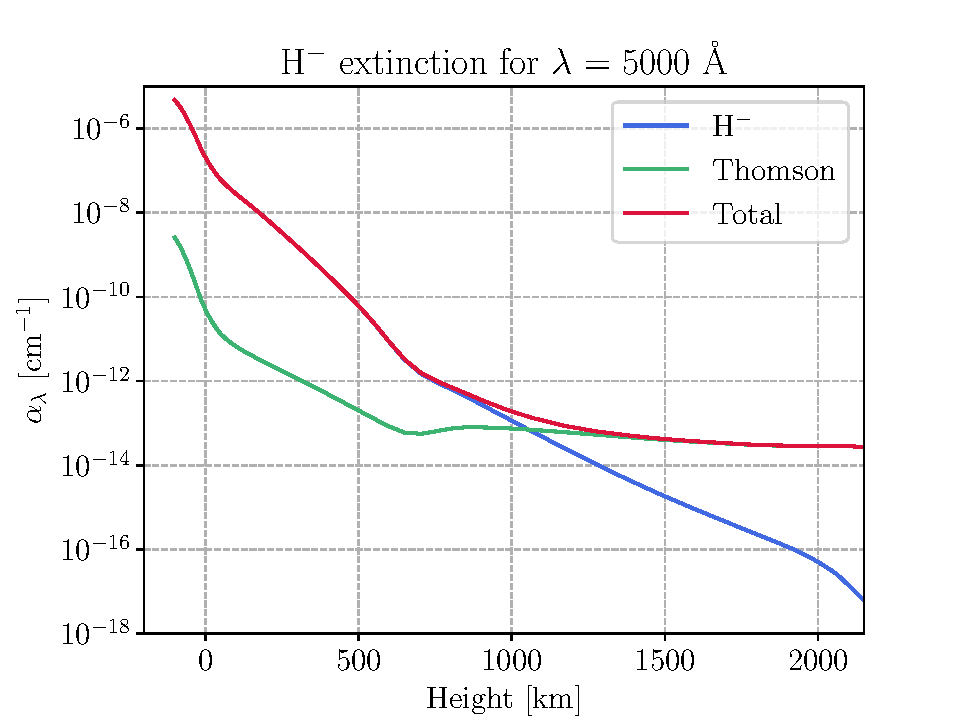
\includegraphics[width = 0.5\textwidth]{figures/2.2/extinction_comparison.pdf}
    \caption{Extinction profiles in the solar atmosphere as a function of height.}
    \label{fig: extinction comp}
\end{figure}
 We observe that the H$^-$ is the dominating extinction for low heights for all of the photosphere and some of the chromosphere. At around $h = 1020$ we see that Thompson scattering surpasses H$^-$ and becomes the dominant extinction contribution. This correlates with the behaviour of the hydrogen number density as seen in figure \ref{fig: FALC number densities} in section 1 where we see that the $n_e$ remains approximately constant where as the $n_H$ continues to drop.
 
 \begin{center}
2.4 \textit{Optical depth}
\end{center}

The extinction profiles are quite valuable. By knowing the stratification  (FALC model) and the continuous extinction as a function of height, we are able to compute the corresponding optical depth scale. This quantity is given by the following expression

\begin{equation}\label{eq: tau}
    \tau_\lambda(h_0) \equiv - \int^{h_0}_\infty \alpha^c_\lambda \;\mathrm{d}h,
\end{equation}
where $h_0$ can be any height.

\begin{figure}[H]
    \centering
    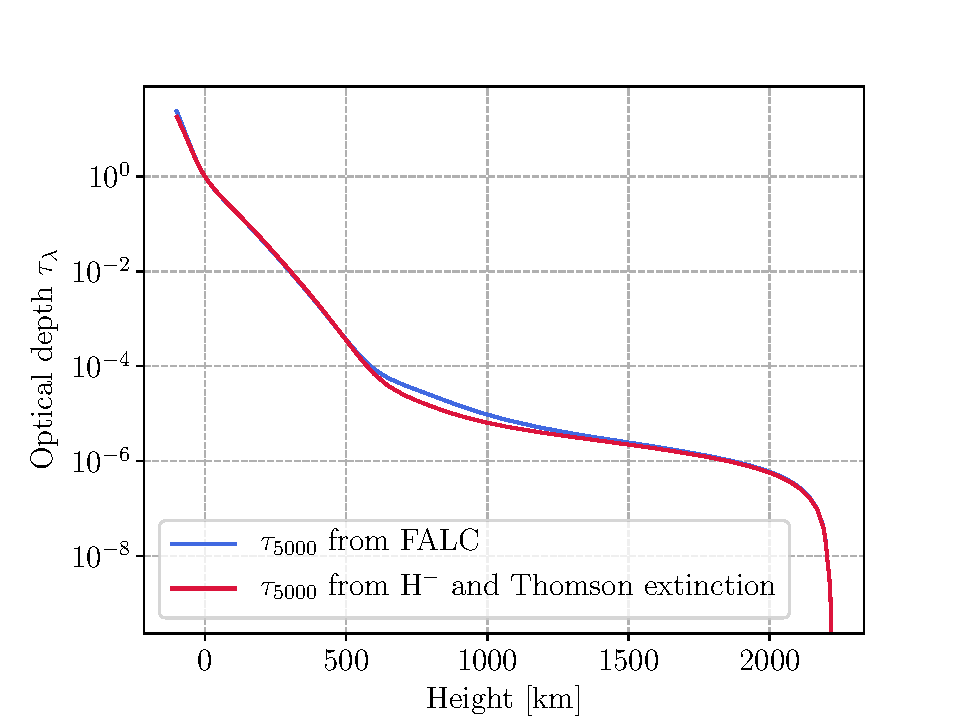
\includegraphics[width = 0.5\textwidth]{figures/2.2/extinction_5000.pdf}
    \caption{The observed optical depth from FALC compared to the numerically calculation. }
    \label{fig : tau5000}
\end{figure}

 By implementing the trapezoidal integration method numerically, we are able to integrate the extinction at $\lambda = 5000 Å$. The resulting optical depth $\tau_{5000}$ is plotted in figure \ref{fig : tau5000}. We find that the observed and computed optical depths corresponds well with each other. We observe a slight deviation between the two curves at the region where the dominating extinction contribution transitions from H$^-$ to Thompson scattering.

 \begin{center}
2.3 \textit{Emergent intensity and height of formation}
\end{center}

The above analysis has readied us to study the intensity which emerges from the center of the solar disk. This intensity is given by

\begin{equation}\label{eq: ilambd}
    I _ { \lambda } = \int _ { 0 } ^ { \infty } S _ { \lambda } \mathrm { e } ^ { - \tau _ { \lambda } } \mathrm { d } \tau _ ,
\end{equation}
where $S_\lambda$ is the source function. It is also interesting to study the intensity contributino function, which is given as

\begin{equation}
\frac { \mathrm { d } I _ { \lambda } } { \mathrm { d } h } = S _ { \lambda } \mathrm { e } ^ { - \tau _ { \lambda } } \alpha _ { \lambda }.
\end{equation}
This function shows the contribution of each layer to the emergent intensity. Its weighted mean is given as

\begin{equation}
    < h > \equiv \frac { \int _ { 0 } ^ { \infty } h \left( \mathrm { d } I _ { \lambda } / \mathrm { d } h \right) \mathrm { d } h } { \int _ { 0 } ^ { \infty } \left( \mathrm { d } I _ { \lambda } / \mathrm { d } h \right) \mathrm { d } h } = \frac { \int _ { 0 } ^ { \infty } h S _ { \lambda } \mathrm { e } ^ { - \tau _ { \lambda } } \mathrm { d } \tau _ { \lambda } } { \int _ { 0 } ^ { \infty } S _ { \lambda } \mathrm { e } ^ { - \tau _ { \lambda } } \mathrm { d } \tau _ { \lambda } }.
\end{equation}

\begin{figure}[H]
    \centering
    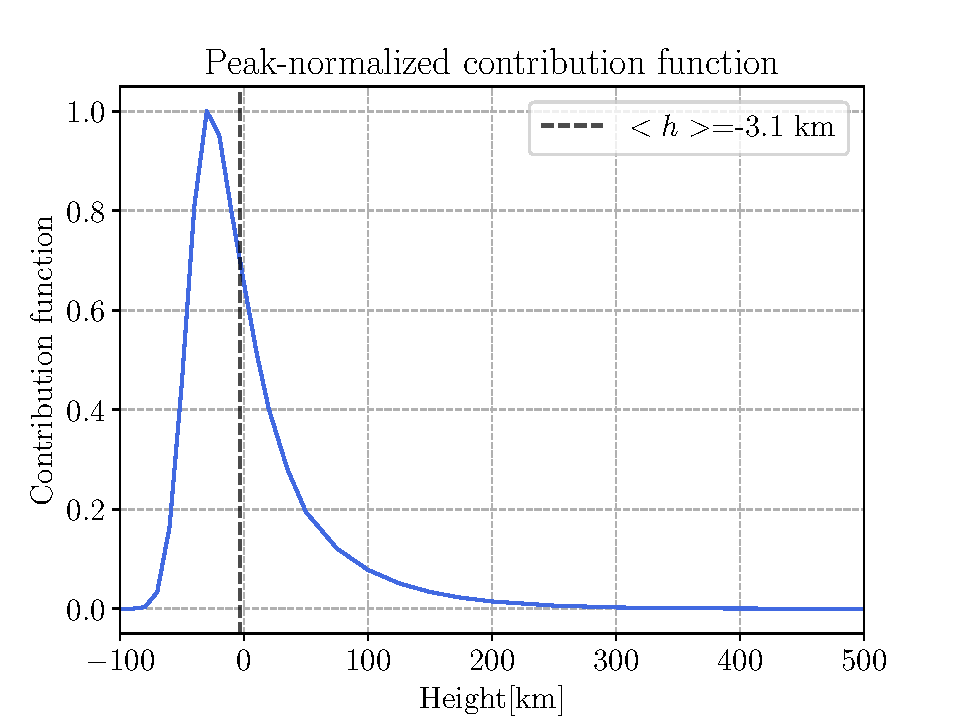
\includegraphics[width = 0.5\textwidth]{figures/2.4/contfunc_single.pdf}
    \caption{The normalized contribution function for the intensity at $\lambda = 5000$Å as a function of height with a mean height of $< h > = -3.1$.}
    \label{fig: peaknorm single}
\end{figure}

We will now study the contribution function in further detail. We start by plotting the peak-normalized contribution function for $\lambda = 5000$Å. The results can be seen in figure \ref{fig: peaknorm single}. The weighted mean height for this wavelength is found to be $< h > = -3.1 $km, which we see deviate from the peak location. We can repeat this exercise for some other wavelengths to compare the behaviour. Computing the Peak-normalized contribution for the wavelengths $\lambda = 1, 1.6$ and $5\;\mu$m gives us the results seen in figure \ref{fig: cont comp}.

\end{multicols}

\begin{table}[H]
\centering
\caption{Comparison of the different computed quantities.  }
\label{tab: 1}
\begin{tabular}{|c|c|c|c|c|l|l|l|}
\hline
$\lambda$ $[\mu$m] & $< h > $ [km] & $h(\tau = 1)$[km] & $T(\tau = 1)$ [K] & $T_b$ [K] & $h(T=T_b)$ [km] & I                     & $B _ { \lambda } \left( T \left[ \tau _ { \lambda } = 1 \right] \right)$ \\ \hline
0.5                & -3.1          & 0                 & 6520               & 6328      & 10              & $4.28 \times 10^{14}$ & $4.67 \times 10^{14}$                                                    \\ \hline
1.0                & 24.1          & 10                & 6340               & 6074      & 30              & $1.25 \times 10^{14}$ & $1.37 \times 10^{14}$                                                    \\ \hline
1.6                & -18           & -30               & 6980               & 6711      & -10            & $4.27\times 10^{13}$  & $4.32 \times 10^{13}$                                                    \\ \hline
5.0                & 76            & 50                & 5790               & 5620      & 75              & $5.74 \times 10^{11}$ & $5.92 \times 10^{1}$                                                     \\ \hline
\end{tabular}
\end{table}

\begin{multicols}{2}

\begin{figure}[H]
    \centering
    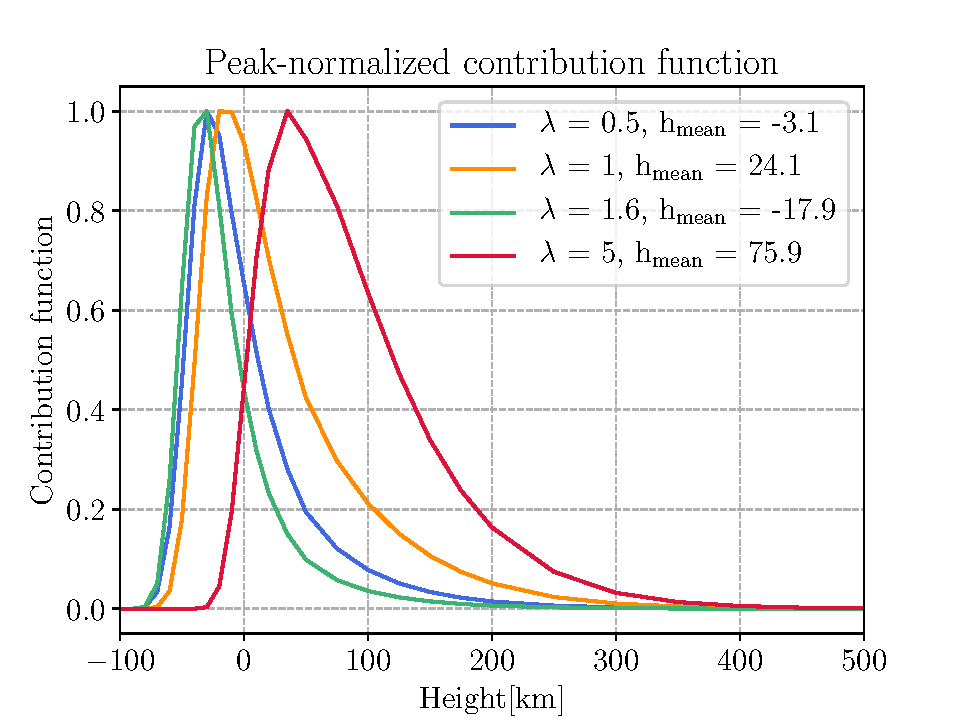
\includegraphics[width = 0.5\textwidth]{figures/2.4/contfunc.pdf}
    \caption{The peak-normalized contribution function for the wavelengths $\lambda = [0.5,\; 1,\; 1.6,\; 5]\mu$m.}
    \label{fig: cont comp}
\end{figure}

We observe that the contribution function values at the locations of $< h >$ creates the familiar shape seen in the brightness temperature of the solar atmosphere suggesting some correlation. We will continue by checking the validity of the LTE Eddington-Barbier approximation. It states the following

\begin{equation}\label{eq: barb}
    I _ { \lambda } \approx B _ { \lambda } \left( T \left[ \tau _ { \lambda } = 1 \right] \right).
\end{equation}
We can then compare the two intensities by finding the temperature where $\tau = 1$ at a given wavelength. This is done by using the various values computed throughout the analysis, and the results can be seen in table \ref{tab: 1}. At $\lambda = 0.5 \mu$m, we find that $I$ and $B_\lambda$ differs by $9.11\%$. Similarly we find the following deviations for the other wavelenghts $\lambda = 1.0 \mu$m : $9.6\%$, $\lambda = 1.6 \mu$m : $1.17\%$ and $\lambda = 1.0 \mu$m : $3.13\%$. All of the intensities are within $10\%$ of the Planck values. Considering the resolution of the data we are working, these values are in good agreement. 

 \begin{center}
2.5 \textit{Disk-center intensity}
\end{center}
We are now able to compute the solar disk-center intensity spectrum by repeating the earlier calculations. We can then compare the intensity from \eqref{eq: ilambd}, with the observed intensity. The results of this comparison is seen below in figure \ref{fig: i comp}. We find that the computed intensity is $I_\lambda^\mathrm{FALC} = 4.29 \times 10^{14}$ erg s$^{-1}$ cm$^{-2}$ ster$^{-1}$ $\mu$m$^{-1}$ which is slightly higher than the observed intensity at $I_\lambda^\mathrm{observed} = 4.08 \times 10^{14}$ erg s$^{-1}$ cm$^{-2}$ ster$^{-1}$ $\mu$m$^{-1}$. This shows that the computed intensity is $5.12\%$ greater than the observed value, suggesting that the model is acceptable. 

\begin{figure}[H]
    \centering
    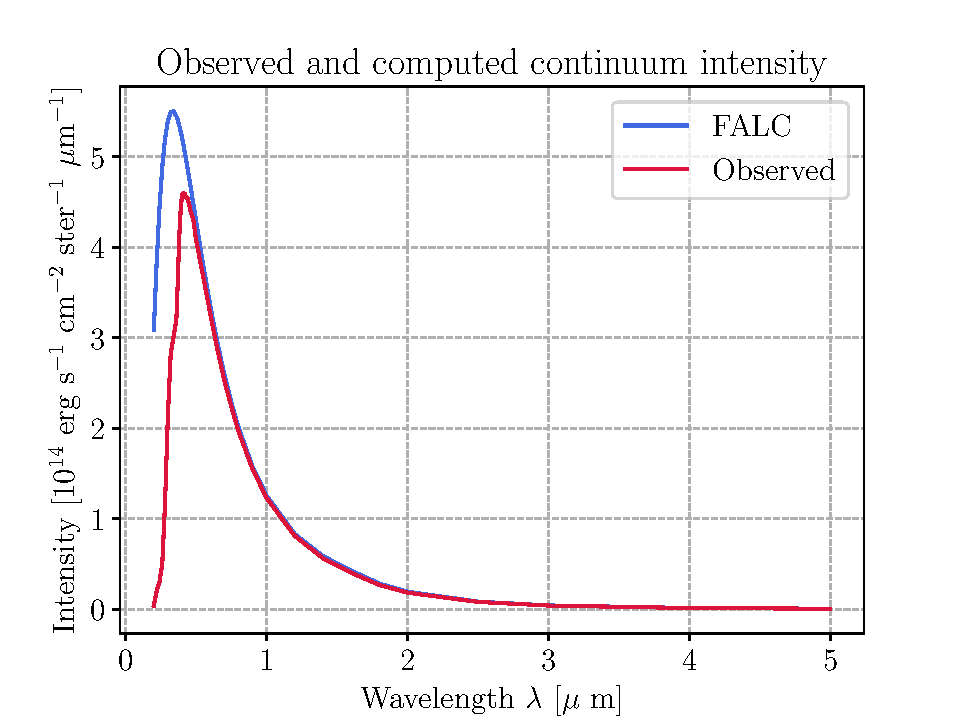
\includegraphics[width = 0.5\textwidth]{figures/2.4/Observed_computed.pdf}
    \caption{The observed and computed emerging intensity from the center of the solar disk as a function of wavelength}
    \label{fig: i comp}
\end{figure}

 \begin{center}
2.6 \textit{Limb darkening}
\end{center}

We can now easily modify the code so that it gives us the intensity which emerges under an angle $\mu = \cos \theta$, in plane-parallel approximation which is given by

\begin{equation}
    I _ { \lambda } ( 0 , \mu ) = \int _ { 0 } ^ { \infty } S _ { \lambda } \mathrm { e } ^ { - \tau _ { \lambda } / \mu } \mathrm { d } \tau _ { \lambda } / \mu.
\end{equation}

We will now repeat the previous intensity evaluation for 10 linearly spaced values of $\mu \in [0,1]$. The results of this calculation can be seen in figure \ref{fig: limb}.
\begin{figure}[H]
    \centering
    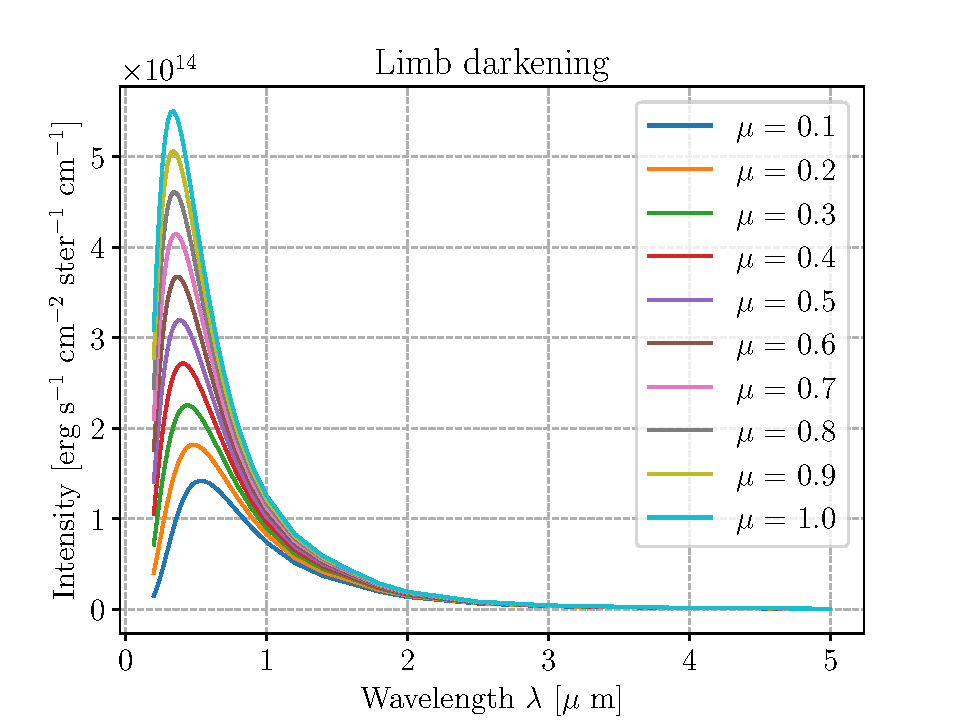
\includegraphics[width = 0.5\textwidth]{figures/2.6/limbdark_wave.pdf}
    \caption{Intensity evaluated for various values of the angle $\mu = \cos \theta$ as a function of wavelength.}
    \label{fig: limb}
\end{figure}

The angle naturally plays a role in the observed intensity, which is seen in \ref{fig: limb} where the intensity decreases as $\mu$ decrease.
We can also plot the normalized intensity as a function of the apparent solar disk $r/R_\Sun = \sin \theta$. This is plotted in figure \ref{fig: norm limb}

\begin{figure}[H]
    \centering
    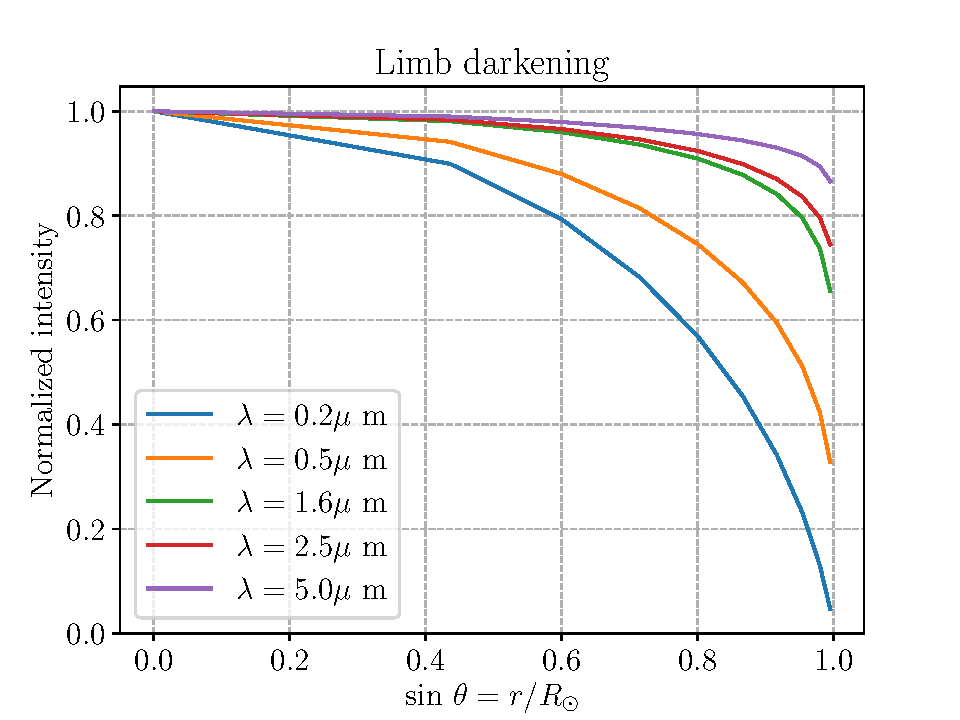
\includegraphics[width = 0.5\textwidth]{figures/2.6/limbdark_rRsun.pdf}
    \caption{The normalized intensity as a function of the apparent solar disk for some selected wavelengths.}
    \label{fig: norm limb}
\end{figure}
We observe that the normalized intensity falls of as we reach the outer edge of the solar disk. This is a result of limb darkening which is an optical effect where the center part of the disk appears brighter than the outer. This can be explained by considering the optical depth. If one assumes that the radiation of the Sun varies linearly with optical depth, then the emerging radiation will be of the intensity at an optical depth of unity. Since the optical depth is a function of our viewing angle, the height at which the optical depth is unity varies as we look across the star, making the outer star look fainter. For specific wavelengths, the opposite can be true in a phenomena called limb brightening. We also observe a variation with wavelength. This is a result of the optical depth being a function of wavelength.

 \begin{center}
2.7 \textit{Flux integration}
\end{center}

The final topic which we will tackle in this part is the astrophysical flux. We are now able to integrate the emergent intensity over emergence angle to get the emergent astrophysical flux, which is given as

\begin{equation}
    F _ { \lambda } ( 0 ) = 2 \int _ { 0 } ^ { 1 } I _ { \lambda } ( 0 , \mu ) \mu \mathrm { d } \mu.
\end{equation}
This expression however becomes a problem as it cant be evaluated at $\mu = 0$. One could use the trapezoidal method as before, but it turns out that this produces too much flux. A better option is to use so the so-called Gaussian quadrature which makes use of orthogonal polynomials. The defining formula is then

\begin{equation}
    \int _ { - 1 } ^ { + 1 } f ( x ) \mathrm { d } x \approx \sum _ { i = 1 } ^ { n } w _ { i } f \left( x _ { i } \right),
\end{equation}
where $x_i$ and $w_i$ are the respective tabulated absicca values and weights. The results of the flux integration can be seen in figure \

\begin{figure}[H]
    \centering
    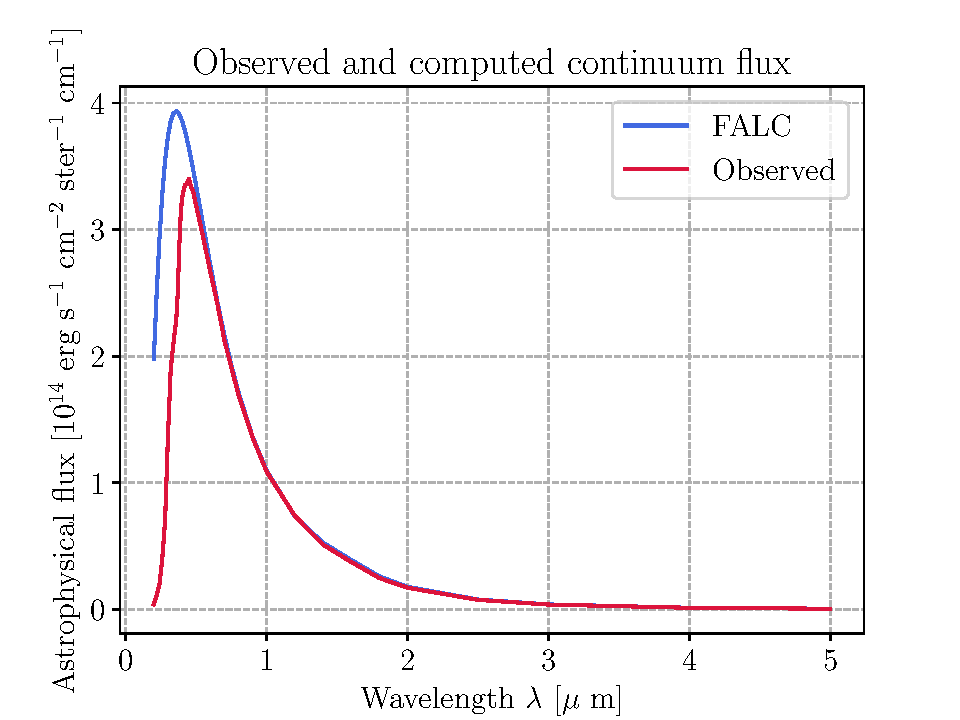
\includegraphics[width = 0.5\textwidth]{figures/2.6/flux_comparison.pdf}
    \caption{Comparison of the numerical astrophysical flux with the observed flux plotted as a function of wavelength.}
    \label{fig: flux}
\end{figure}

We observe a good accordance between the numerically computed flux and the observed flux, similar to the previous intensity comparison.

 \begin{center}
2.8 \textit{Conclusion to part 2}
\end{center}

Most of the results have been discussed through out the report. We will however provide a short summary. We started by studying the solar continuum. We found that the continuum was a good match with certain Planck fits. We followed that up by studying H$^-$ extinction, where we learned that the brightness temperature derived from the Planck function could help explain the observed behaviour. Further extinction studies showed that the dominating extinction process in the solar atmosphere is H$^-$ at low heights, while Thompson scattering dominates the higher altitudes. 

We continued by looking at contribution functions for different wavelengths where we found that the mean heights $< h >$ was a good approximation to the height where $T = T_b$. We also saw that the Eddington-Barbier approximation holds the lower solar atmosphere as the observed intensity deviated by less than $10\%$ of the predicted black body intensity at $T[\tau = 1]$. It should be noted that LTE is not valid for Thompson scattering. 
We finished by looking at the limb darkening phenomena, where the saw the effect of the angle dependence of the emergent intensity.

 
\begin{center}
3. \textsc{Spectral lines from the solar atmosphere}
\end{center}

We will now move our attention to the formation of spectral lines with a focus on the formation of the Na I D$_1$ line at $\lambda = 589$nm. Below is some figures considering the Na I D spectral lines and the Boltzmann and Saha distributions. I could not find time to complete the rest of the exercises.

\begin{figure}[H]
    \centering
    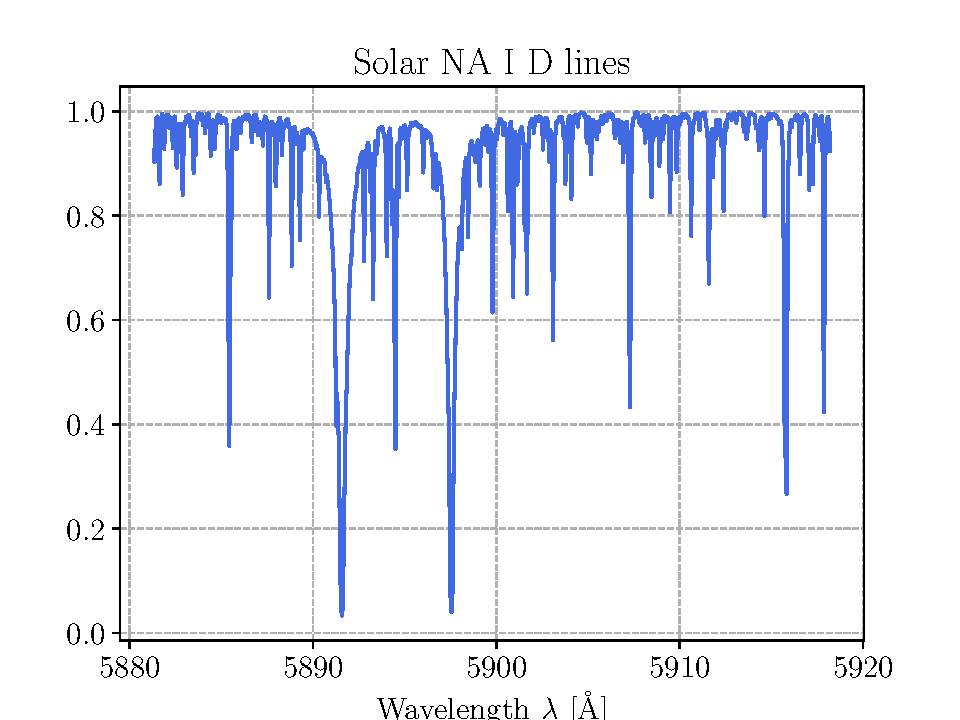
\includegraphics[width = 0.5\textwidth]{figures/3/solarspectran.pdf}
    \caption{The spectrum of the sun in the wavelength range $\lambda \in [5800, 5920]Å$. The two Na I D lines are clearly visible.}
    \label{fig: 3.1}
\end{figure}

\begin{figure}[H]
    \centering
    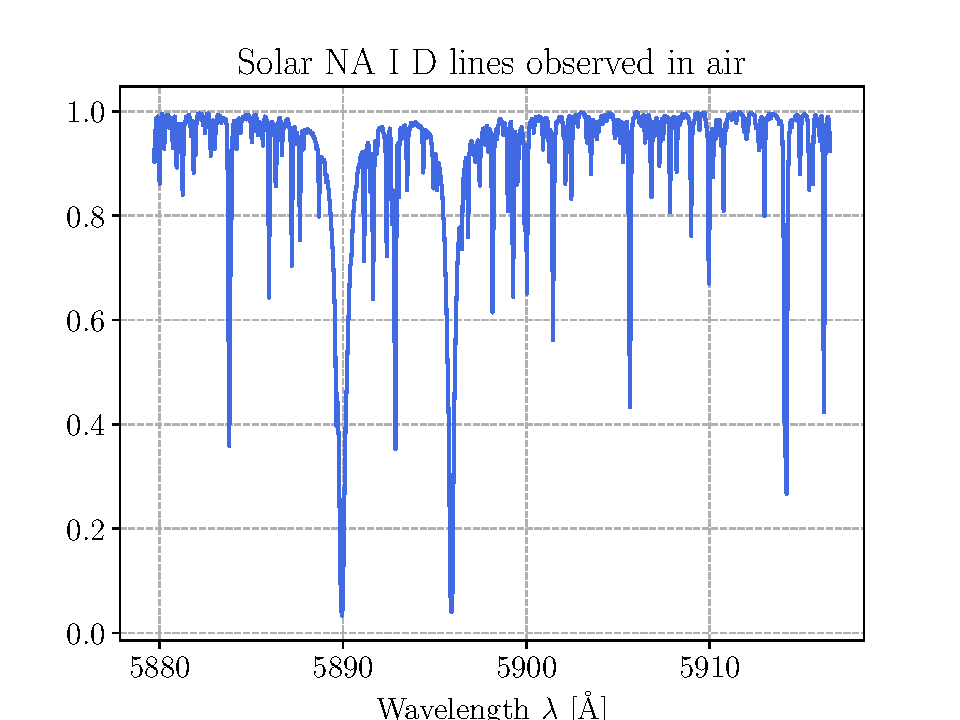
\includegraphics[width = 0.5\textwidth]{figures/3/solarspectranair.pdf}
    \caption{The spectrum of the sun in the wavelength range $\lambda \in [5800, 5920]Å$. We notice that the spectral lines has been shifted to the left as a result of the viewing in air.}
    \label{fig: 3.2}
\end{figure}

\begin{figure}[H]
    \centering
    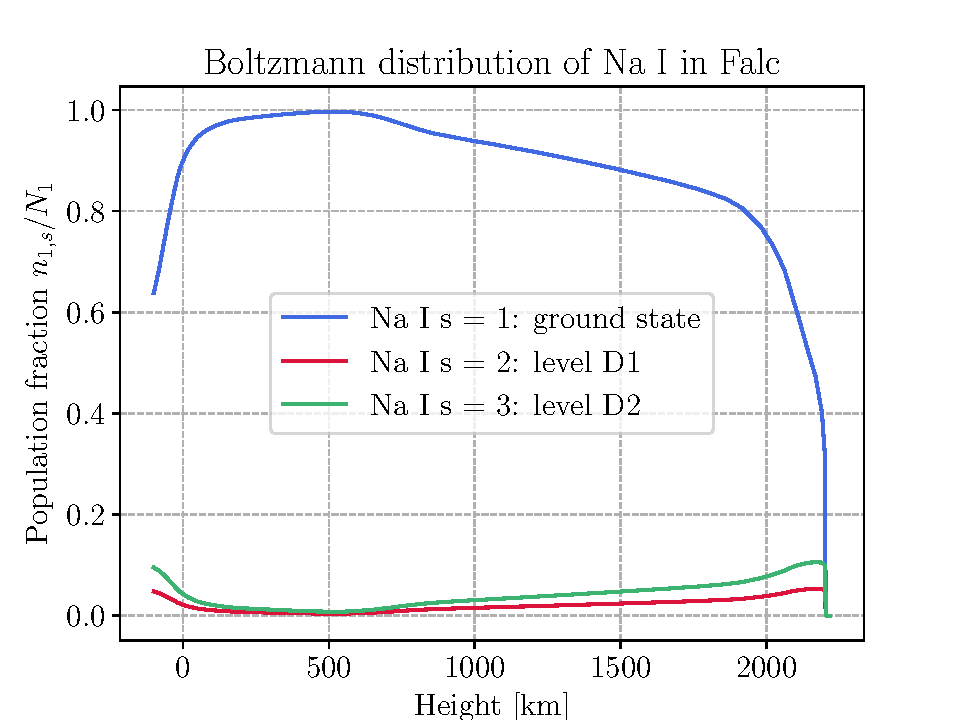
\includegraphics[width = 0.5\textwidth]{figures/3/boltz.pdf}
    \caption{The Boltzmann distribution of Na I as a function of height. We observe that the ground state $s=1$ population dominates throughout most of the solar atmosphere. We do see an increase in higher energy states as the temperature increase at the lower and higher ends. The population of Na I $s = 1$ drops to 0 at the transition to the corona. This is likely because of the high temperatures.}
    \label{fig: 3.3}
\end{figure}

\begin{figure}[H]
    \centering
    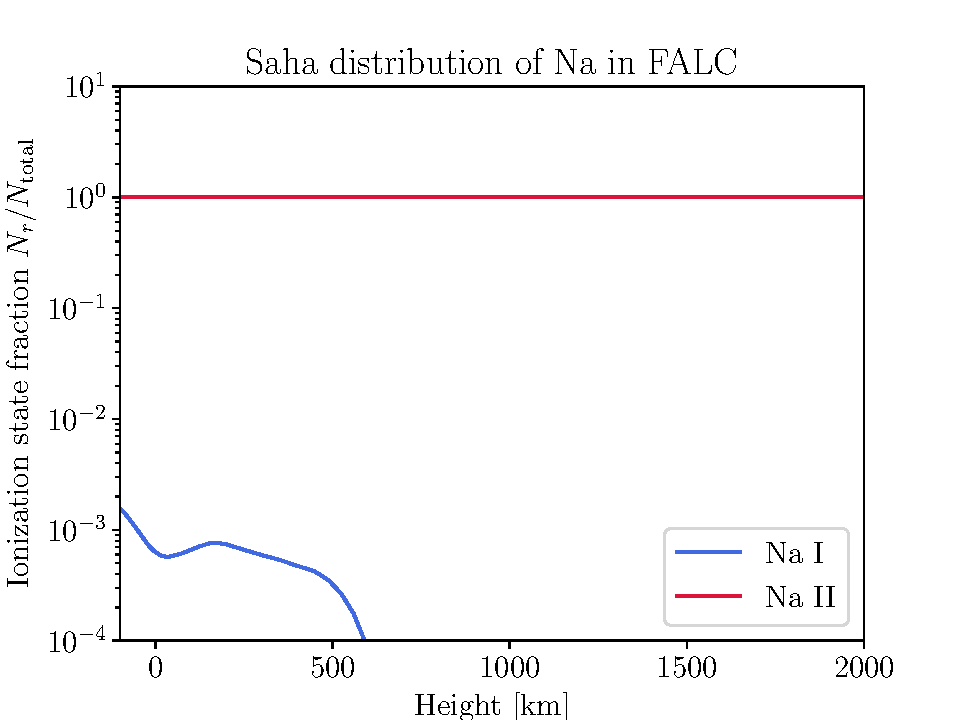
\includegraphics[width = 0.5\textwidth]{figures/3/saha.pdf}
    \caption{The Saha distribution of Na I as a function of height. We note that there are hardly any Na I in the solar atmosphere, as most of it is ionized to Na II.}
    \label{fig: 3.4}
\end{figure}



\end{multicols}


\end{document}